%!TEX root = report.tex
\newcommand{\R}{\mathbb{R}}
\section{Methodology}
\label{Sec:methodology}

%Methodology/Algorithm: What method or algorithm are you proposing? If there are existing implementations, will you use them and how? How do you plan to improve or modify such implementations?

Our model will start from the state-of-the-art convolutional neural network model. Upon CNN baseline, we modify it with a author embedding activation layer. 
\subsection*{CNN Baseline}
Sentence word embeddings are concatenated together as inputs, $(\mathbf{h_1},\mathbf{h_2},\ldots,\mathbf{h_n})$, where the maximum sentence length is usually less than $n$ words due to character constraints of tweets. If a sentence is less than $n$ words, we will use zero word vectors to fill it. Therefore, our input data are consistent length $n$. Next, a convolutional layer is performed on the sentence word embeddings with a width-two window to $d$-channel filters of size $n-1$. Then a max pooling layer pick the largest value among the $n-1$ layers to form a $d$-channel features. Finally, this length $d$ features are input into a softmax layer to classify three-class label. To express the above model structures in mathematical equation:
\begin{enumerate}
	\item The convolutional layer:
\begin{equation}
	\mathbf{c_i} = \tanh(W_L\mathbf{h_i} + W_R \mathbf{h_{i+1}} + \mathbf{b}), i=1,2,\ldots,n-1
\end{equation}
where $\mathbf{h_i}\in \R^{D\times1}$ are word embedding, $\mathbf{c_i} \in \R^{d\times1}$ are padding $i$ in the convolutional layer, $W_L$ and $W_R$ are convolutional layer kernel matrices, $\mathbf{b}$ is the convolutional layer bias vector.
\item The max pooling layer:
\begin{equation}
	\mathbf{s} = \max_{i=1,2,\ldots,n-1}\mathbf{c_i}
\end{equation}
where $\mathbf{s} \in \R^{d \times 1}$ are features learned from CNN.
\item The softmax layer:
\begin{equation}
	\mathbb{P}(Y=c|s)=\frac{\exp(W_{c}\mathbf{s}+\mathbf{b_c})}{\sum_{c'}\exp(W_{c'}\mathbf{s}+\mathbf{b_c'})}
\end{equation}
\end{enumerate}

\begin{figure}[h]
\centering
\begin{minipage}{.5\textwidth}
  \centering
  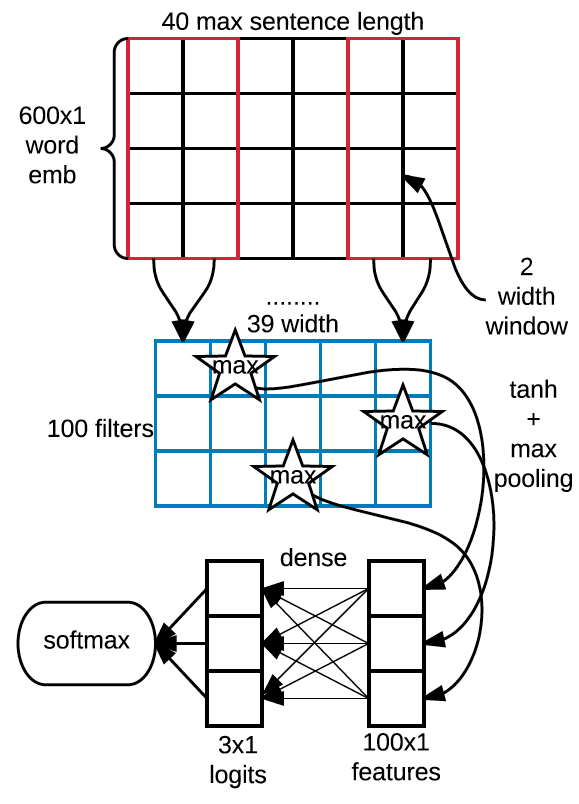
\includegraphics[width=1\linewidth]{cnn}
    \label{fig:cnn}
\end{minipage}%
\caption{baseline CNN network strucutre}
\end{figure}

\subsection*{Author Activated CNN}
In our dataset, each tweet also includes a user ID. We use algorithm of LINE, DeepWalk and Node2Vec to learn a network node embedding for each user ID to form author embeddings $\mathbf{a}$ for each sentence $(\mathbf{h_1},\mathbf{h_2},\ldots,\mathbf{h_n})$. Compared to baseline CNN, we use one hidden layer to learn an activated vector $\mathbf{z}$ for each user which element-wise multiplies convolutional layer. The intuition behind this activated vector is that for each convolutional channel, different user may display different behaviors. This is in fact equivalent with bilinear form with low rank approximation. We can exploit the interaction between word embeddings and author embeddings. To express the above model structures in mathematical equation:
\begin{enumerate}
	\item The convolutional layer:
\begin{equation}
	\mathbf{c_i} = \tanh(W_L\mathbf{h_i} + W_R \mathbf{h_{i+1}} + \mathbf{b}), i=1,2,\ldots,n-1
\end{equation}
where $\mathbf{h_i}\in \R^{D\times1}$ are word embedding, $\mathbf{c_i} \in \R^{d\times1}$ are padding $i$ in the convolutional layer, $W_L$ and $W_R$ are convolutional layer kernel matrices, $\mathbf{b}$ is the convolutional layer bias vector.
\item The user activated layer:
\begin{equation}
	\mathbf{z} = \tanh(W_a\mathbf{a}  + \mathbf{b_a})
\end{equation}
where $\mathbf{z} \in \R^{d \times 1}$ are activation features learned from author embeddings $\mathbf{a} \in \R^{A\times1}$.
\item The max pooling layer with user activation:
\begin{equation}
	\mathbf{s} = \max_{i=1,2,\ldots,n-1}\mathbf{z}\odot\mathbf{c_i}
\end{equation}
where $\mathbf{s} \in \R^{d \times 1}$ are features learned from CNN.
\item The softmax layer:
\begin{equation}
	\mathbb{P}(Y=c|s)=\frac{\exp(W_{c}\mathbf{s}+\mathbf{b_c})}{\sum_{c'}\exp(W_{c'}\mathbf{s}+\mathbf{b_c'})}
\end{equation}
\end{enumerate}
Note that the difference between node activated CNN and baseline CNN is that activated CNN has new parameters $W_a$ and $\mathbf{b_a}$. In fact, originally we would like to build bilinear form for each word vector $\mathbf{h_i} W_{ha} \mathbf{a}$ to form some interaction features for each word, hoping the interaction features could help identify different behaviors for each user community. But we find out our data sample is too small to learn this bilinear matrices $W$, therefore we have to use some low rank approximation of $W$ which can be equivalent to element-wise activation as described above.

%\begin{figure}[htbp] %  figure placement: here, top, bottom, or page
%   \centering
%   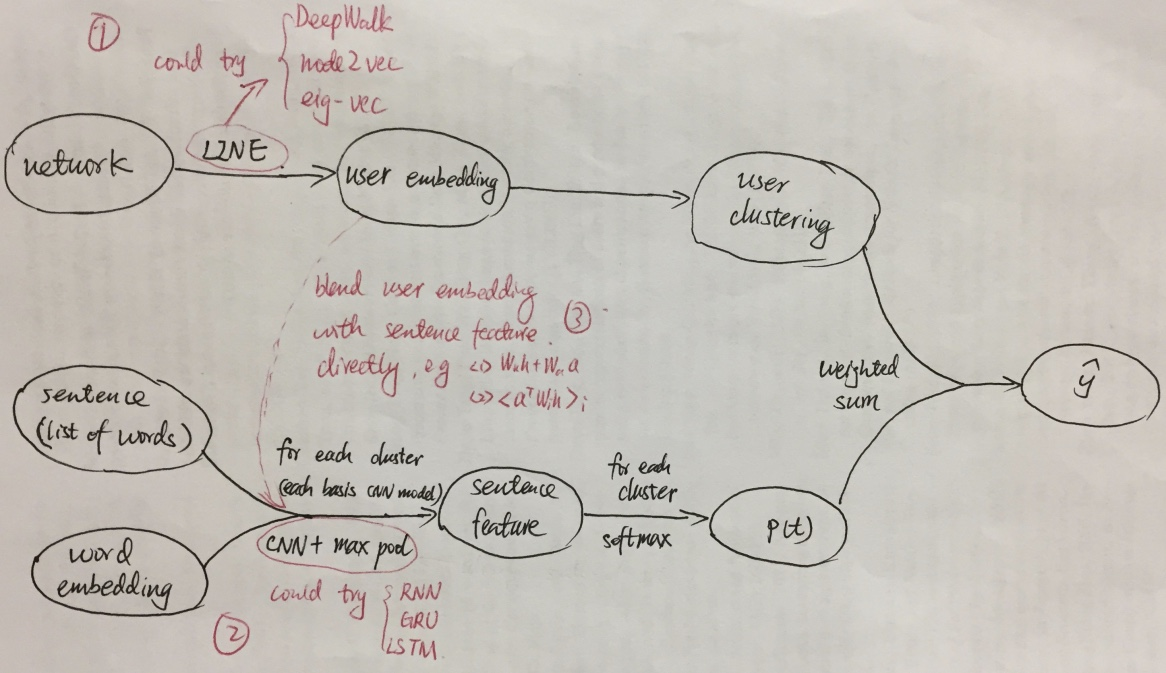
\includegraphics[width=5.2in]{flow.jpg} 
%   \caption{General Methodology}
%   \label{Fig:Flow}
%\end{figure}


%
%We are going to extend this model in three aspects, as is illustrated in the red lines in Figure \ref{Fig:Flow}. To be specific, 
%\begin{enumerate}   [(1)]
%%\setcounter{enumi}{3}
%\item Using other node embedding methods in network analysis, such as \textit{DeepWalk}[2] and \textit{node2vec}[3];
%\item Explore other methods to combine author information and sentence information, especially the bilinear form $a^T W h$ which measures the interaction between author and sentence. Here $a$ is the author embedding and $h$ is the sentence embedding.
%\item Explore other models in sentiment analysis, such as RNN, GRU, and LSTM.
%\end{enumerate}
